\documentclass[12pt, a4paper]{siweb}
\usepackage{xeCJK}
\setCJKmainfont{PingFang TC}
\usepackage{hyperref}

\usepackage{tikz}

\makeatletter
\renewcommand{\thesection}{\@arabic\c@section}
\makeatother

\title{Map Editor}
\author{Si manglam}
\setcounter{tocdepth}{3}
\begin{document}
\maketitle
\tableofcontents
\newpage
\pagenumbering{arabic}
\linespread{1.35}
\section{前言}

這是一篇解釋 Map Editor 是怎麼寫的,以及為什麼要這樣寫的解釋文章,文章內容不只注重於解釋,也會花點篇幅去評論程式碼,說這樣寫的好處與壞處分別為何,而我是經過怎麼樣的權衡後才下決定的。事不宜遲,就讓我們開始吧!

\section{概覽}

在談論如何使用工具之前,我們必須知道自己的目標到底是什麼?這裡很明確的,是一個編輯地圖的軟體。那他有什麼需求?這是第二個問題,我們要列需求表出來,因為即使有工具,沒有方向還是做不出東西來。下面是我列的需求:

\begin{itemize}
\item 需要一個 GUI (使用者圖形介面)來方便操作。
\item 需要接收滑鼠輸入,在滑鼠點擊時把物體放在當前位置上。
\item 需要用一個方式把當前的地圖轉換成檔案。
\end{itemize}

將這些要求都列出來後,就可以開始構思可以用甚麼工具去達成這些效果。以及這些功能要多完善。像是 GUI 要接收什麼?需要有一套複雜的 Icon 與視窗嗎?需要讓所有功能在 GUI 上佔有一席之地嗎?這些都是需要思考的問題。

因為當初是希望快速做出一個簡單的 Demo,並且將簡單放在比好維護更優先的位置,所以不希望用太複雜的方式去寫,也不需要寫出過於複雜、龐大 GUI 系統。

這樣就只需要一個介面,然後使用者輸入也從簡,只接收鼠標點擊與一個鍵盤輸入,力求在最短時間內寫完這個。

\subsection{程式架構}

既然我們已經把需求都列好了,接下來就得開始思考我們需要怎樣的程式去完成這些需求?我們是用 pygame 實作,並且這個專案是希望可以讓他人也學會 pygame,所以在考慮時最細節是需要以製作遊戲的角度去思考,而不能用製作 App 的角度去想。

一個遊戲會由以下幾個組件組成:

\begin{itemize}
\item 事件處理
\item 碰撞
\item 畫面渲染
\end{itemize}

所以我們寫出的程式結構應該會像下圖所示:

\begin{siweb}{main.py}
\begin{mylisting}{main.py}
import pygame, json
pygame.init()
<<物件定義>>
<<全域變數>>
<<遊戲主迴圈>>
\end{mylisting}
\label{main.py_0}\label{物件定義_father}\label{全域變數_father}\label{遊戲主迴圈_father}

\end{siweb}

有了大致的架構就可以來著手實作了!

\section{遊戲主迴圈}

遊戲主迴圈是遊戲最重要的部分,他會定義遊戲每一幀之間的更新流程。我們這個軟體沒有很複雜,每一幀之間需要做的就只有處理滑鼠與鍵盤輸入,不需用去做物理運算之類的東西。所以我們的主迴圈會長得像以下這樣:

\begin{siweb}{遊戲主迴圈}
\begin{mylisting}{遊戲主迴圈}
while running:
	<<事件迴圈>>
		
	<<渲染更新>>
\end{mylisting}
\label{遊戲主迴圈_0}\label{事件迴圈_father}\label{渲染更新_father}
父區塊在第\pageref{遊戲主迴圈_father} 頁
\end{siweb}

分別處理完事件後,再去處理畫面渲染。這裡用 while 迴圈是為了讓這個迴圈不斷的執行,畢竟遊戲是需要一直跑的,直到接收到關閉事件。這裡用的方式是設一個全域變數 running,讓整個程式碼可以更加清楚明瞭。如果只用 while,便無法達成這個效果。

\begin{siweb}{全域變數}
\begin{mylisting}{全域變數}
running = True
\end{mylisting}
\label{全域變數_0}
父區塊在第\pageref{全域變數_father} 頁\\參見第\pageref{全域變數_0}, \pageref{全域變數_1}, \pageref{全域變數_2}, \pageref{全域變數_3}, 頁
\end{siweb}

\subsection{事件處理}

先讓我們從事件處理開始。事件在 pygame 內可以用 \verb|pygame.event.get()| 來取得目前所有的事件,並且會以 List 的方式回傳,所以我們可以用 for 迴圈去跑過所有 event,並讓遊戲根據不同的 event 做出不同的回應。

\begin{siweb}{事件迴圈}
\begin{mylisting}{事件迴圈}
for event in pygame.event.get():
	<<處理關閉事件>>
	<<處理鍵盤事件>>
	<<處理滑鼠事件>>
\end{mylisting}
\label{事件迴圈_0}\label{處理關閉事件_father}\label{處理鍵盤事件_father}\label{處理滑鼠事件_father}
父區塊在第\pageref{事件迴圈_father} 頁
\end{siweb}

事件迴圈建立好後,就可以開始根據不同事件撰寫處理流程。第一個要說的還是關閉事件,畢竟遊戲可以不能玩,但一定要可以關起來,不然就只能強制關機了。

\subsubsection{關閉事件}

在 pygame,事件類型是被定義為 \verb|pygame.事件名稱|,像是關閉視窗的事件就被定義為 \verb|pygame.QUIT|,所以我們可以用 if 條件式去判斷當前事件。

\begin{siweb}{處理關閉事件}
\begin{mylisting}{處理關閉事件}
if event.type == pygame.QUIT:
	running = False
	pygame.quit()
\end{mylisting}
\label{處理關閉事件_0}
父區塊在第\pageref{處理關閉事件_father} 頁
\end{siweb}

以上是判斷關閉事件與處理關閉事件的方法。如果在事件迴圈內,有一個關閉事件,那就把 running 改為 False,並呼叫 \verb|pygame.quit()| 函數關閉遊戲。

\subsubsection{滑鼠事件}

再來,先讓我們處理滑鼠事件。我的想法是滑鼠只要一點,就會在當前位置上放一個方塊。這些方塊會被儲存在一個 list 裡面,會需要被儲存是因為每一幀都要先畫出這些方塊,所以需要找一個方式去儲存他們。

\begin{siweb}{處理滑鼠事件}
\begin{mylisting}{處理滑鼠事件}
if event.type == pygame.MOUSEBUTTONDOWN:
	pos_x, pos_y = event.dict["pos"]
	<<偵測當前滑鼠位置是否有與其他方塊碰撞>>
	<<加入方塊>>
\end{mylisting}
\label{處理滑鼠事件_0}\label{偵測當前滑鼠位置是否有與其他方塊碰撞_father}\label{加入方塊_father}
父區塊在第\pageref{處理滑鼠事件_father} 頁
\end{siweb}

如果滑鼠按鈕被按下,那就會先得到當前的滑鼠位置,並利用目前的滑鼠位置去偵測是否有其他方塊與滑鼠碰撞,不然如果重複加入就會產生過多的冗余資料。在確認沒有其他方塊時,才會加入方塊。

\subsubsection{一點點的物件導向}

再繼續往下走之前,我們需要先來定義方塊這個物件。為什麼要用物件?因為物件可以幫我們把該物體的資訊都綁在一起,讓我們寫 code 時可以不用用過多的變數去儲存相關的資訊。

聽起來很難理解,但我相信在一段時間的實作後,你們就可以了解 OOP 的好處了。所以讓我們先來定義這個物件吧!

\begin{siweb}{物件定義}
\begin{mylisting}{物件定義}
class BaseMapObject(pygame.sprite.Sprite):
	def __init__(self, pos_x, pos_y):
		self.image = pygame.surface.Surface((50, 50))
		self.rect = self.image.get_rect(topleft = (pos_x, pos_y))
		self.image.fill("black")
		
\end{mylisting}
\label{物件定義_0}
父區塊在第\pageref{物件定義_father} 頁
\end{siweb}

物件導向這邊,我也不太會解釋,但我會盡我所能的去解釋。在 python 裡面 class 是宣告物件的保留字,而括號內的則是繼承哪個類別。繼承是 OOP 內的一個概念,來自維基百科的解釋如下:「繼承可以使得子類別具有父類別的各種屬性和方法,而不需要再次編寫相同的程式碼。」非常繞口,所以我找了一篇\href{https://medium.com/程式愛好者/什麼是oo-物件導向與繼承-6955239576af}{文章},希望可以幫忙解釋。

\verb|__init__()| 函數是 python 中的特殊函數,其指建立物件時執行的初始化函數。這個函數會接收三個參數 \verb|self, pos_x, pos_y|,其中 self 是由 python 自動帶入,所以這裡可以暫時忽略他。剩下的 \verb|pos_x, pos_y| 則是會賦予給 rect 自動產生座標。

整個初始化流程如下:

\begin{enumerate}
\item 創建一個叫 image 的 members(成員,這是專有名詞)其為 25 X 25 像素的 Surface (表面,之後會細細解釋)
\item 創建一個叫 rect 的 member 並讓這個 rect 的左上角等於傳進去的參數。
\item 最後把 image 用黑色填滿。
\end{enumerate}

這樣子就得到了一個簡單的、封裝了資訊的物件。可以用這個物件來降低複雜度!!

\subsubsection{加入方塊}

先讓我們撰寫加入方塊的程式碼,這邊需要記得,遊戲是像素風格的,並且遊戲內每個物體的大小目前暫定為 $50 \times 50$,所以每個方塊的座標都應該是 50 的倍數。加入的方塊會以 list 的方式儲存起來,雖說這並不一個好主意,但勝在簡單,所以這裡演示教學是用這個方式:

\begin{siweb}{加入方塊}
\begin{mylisting}{加入方塊}
if not collide:
	terrain_group.append(BaseMapObject(int(pos_x / 50) * 50, int(pos_y / 50) * 50))
\end{mylisting}
\label{加入方塊_0}
父區塊在第\pageref{加入方塊_father} 頁
\end{siweb}

這邊是用 append 的方式把新的 BaseMapObject 給加進 list,位置則是會被除以 50 後並轉換成整數(無條件捨去)然後再乘以 50,這樣就能確保座標一定是 50 的倍數。

\begin{siweb}{全域變數}
\begin{mylisting}{全域變數}
terrain_group = []
\end{mylisting}
\label{全域變數_1}
父區塊在第\pageref{全域變數_father} 頁\\參見第\pageref{全域變數_0}, \pageref{全域變數_1}, \pageref{全域變數_2}, \pageref{全域變數_3}, 頁
\end{siweb}

\subsubsection{碰撞偵測}

碰撞偵測是個很複雜的領域,他牽涉到一大堆複雜的演算法與複雜數學。想要寫好碰撞偵測是一件很難的事情,所幸 pygame 提供了一些已經寫好的碰撞偵測讓我們使用,這樣就不用從頭寫了!

在講碰撞偵測之前,可能需要先簡單的帶一下 rect 這個東西。rect 在 pygame 裡可以想像成一個 surface 的碰撞箱,他記錄著這個 surface 的 xy 座標與長寬資訊,所有的碰撞偵測都需要用 rect 提供的方法來做偵測。

除此之外,rect 也定義了許多不同的點,讓我們可以更加準確去放置當前的 surface。詳細提供的點如下圖所示:

\begin{center}
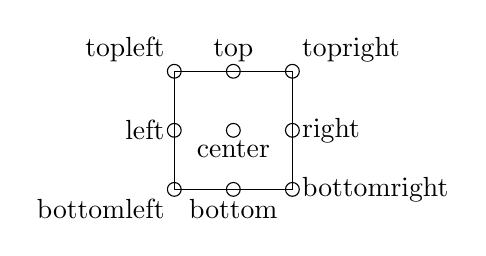
\begin{tikzpicture}[x = 0.25cm, y = 0.25cm]
\draw (-3, -3) rectangle (3, 3);
\draw (-3, -3) circle (0.35) node[below left] {bottomleft};
\draw (-3, 0) circle (0.35) node[left] {left};
\draw (-3, 3) circle (0.35) node[above left] {topleft};
\draw (0, 3) circle (0.35) node[above] {top};
\draw (3, 3) circle (0.35) node[above right] {topright};
\draw (3, 0) circle (0.35) node[right] {right};
\draw (3, -3) circle (0.35) node[below, right] {bottomright};
\draw (0, -3) circle (0.35) node[below] {bottom};
\draw (0, 0) circle (0.35) node[below] {center};
\end{tikzpicture}
\end{center}
\newpage

\begin{siweb}{偵測當前滑鼠位置是否有與其他方塊碰撞}
\begin{mylisting}{偵測當前滑鼠位置是否有與其他方塊碰撞}
collide = False
for block in terrain_group:
	if block.rect.collidepoint((pos_x, pos_y)):
		collide = True
		break
\end{mylisting}
\label{偵測當前滑鼠位置是否有與其他方塊碰撞_0}
父區塊在第\pageref{偵測當前滑鼠位置是否有與其他方塊碰撞_father} 頁
\end{siweb}

\verb|collidepoint| 是 pygame 用來偵測一點是否在該 rect 內的方式,我們先偵測滑鼠點擊區域內是否有 block 在。如果有,那就把 collide 設為 True 並不再偵測,讓後面加入方塊 \ref{加入方塊_0} 自行去判斷是否該加入方塊。

\subsection{渲染更新}

承接上面介紹儲存地形方塊,這裡來講如何將他們渲染到顯示視窗上。這部分會補充前面有稍稍提到 surface 的概念,並更近一步的深入講解。surface 在 pygame 內可以想像為一件事物的表面,可能是 GUI、可能是角色,所有可以被顯示出的東西都會有這個屬性。

最簡單的創建一個 surface 的方法就是利用 \verb|pygame.surface.Surface| 的方式去創建 surface(詳見第\pageref{物件定義_0}頁)。一般的、非與顯示器直接連接的 surface 都可以用這個方式去創建。如果是與主 surface 也就是與顯示器直接連接的,就必須用 \verb|pygame.display.set_mode| 的方式去建立,需注意在 pygame 只能有一個主 surface。

\begin{siweb}{全域變數}
\begin{mylisting}{全域變數}
display_surface = pygame.display.set_mode((0, 0), pygame.FULLSCREEN)
\end{mylisting}
\label{全域變數_2}
父區塊在第\pageref{全域變數_father} 頁\\參見第\pageref{全域變數_0}, \pageref{全域變數_1}, \pageref{全域變數_2}, \pageref{全域變數_3}, 頁
\end{siweb}

獲得了主 surface 後,我們就可以把 \verb|terrain_group| 裡的 block 一個個拿出來渲染到主 surface 上,這裡一樣用 for 迴圈去寫。一樣的,我需要在這裡說,這並不是一個好的方式,只是比較基礎,所以在這裡用這個方式,不然可以用一些更簡單的方法去寫。

\begin{siweb}{渲染更新}
\begin{mylisting}{渲染更新}
display_surface.fill('white')
for block in terrain_group:
	display_surface.blit(block.image, block.rect)
pygame.display.update()
\end{mylisting}
\label{渲染更新_0}
父區塊在第\pageref{渲染更新_father} 頁
\end{siweb}

渲染更新的流程也很簡單,先把 \verb|display_surface| 上填滿白色,再將 \verb|terrain_group| 內的方塊一個個拿出來渲染到主畫面上。blit 是指將一個表面渲染到另一個表面的方法,他需要用座標去指定渲染的位置,但在這裡我們用 rect 去指定。

\section{鍵盤事件}

\subsection{輸出地圖}

繞了一圈之後終於可以跳回來講輸出檔案的方式了,我們希望地圖是可以被儲存在 json 檔的格式,這邊可以借助 json module 的幫助,他可以將 python 的資料型態轉換成 json 的資料格式。

\begin{siweb}{處理鍵盤事件}
\begin{mylisting}{處理鍵盤事件}
if event.type == pygame.KEYDOWN:
	if event.key == pygame.K_e:
		output['level'] = "Test"
		output['size'] = 50
		output['mapdata'] = []
		for block in terrain_group:
			output['mapdata'].append({"x" : block.rect.x, "y" : block.rect.y, "type" : type_dict[type(block)]})
		with open("level.json", "w+") as f:
			json.dump(output, f)
\end{mylisting}
\label{處理鍵盤事件_0}
父區塊在第\pageref{處理鍵盤事件_father} 頁\\參見第\pageref{處理鍵盤事件_0}, \pageref{處理鍵盤事件_1}, 頁
\end{siweb}

這裡需要學一點 json 檔才能知道這裡在幹嘛,但很簡單,所以不在此贅述。這裡比較有趣的是 \verb|type_dict| 的使用,這裡是以該物件的類型作為 key 然後與定義其對應的 value 讓遊戲在解讀時可以知道他到底是什麼。

\begin{siweb}{全域變數}
\begin{mylisting}{全域變數}
output = {}
type_dict = {
	type(BaseMapObject(0, 0)) : "ground"
}
\end{mylisting}
\label{全域變數_3}
父區塊在第\pageref{全域變數_father} 頁\\參見第\pageref{全域變數_0}, \pageref{全域變數_1}, \pageref{全域變數_2}, \pageref{全域變數_3}, 頁
\end{siweb}

\subsection{其他退出方式}

因為全螢幕時會無法按到關閉視窗的叉叉,所以我會幫 esc 鍵加上退出遊戲的功能。這裡就與之前寫退出事件時一樣,只不過感測的對象改成 esc 鍵而已。

\begin{siweb}{處理鍵盤事件}
\begin{mylisting}{處理鍵盤事件}
	if event.key == pygame.K_ESCAPE:
		running = False
		pygame.quit()
\end{mylisting}
\label{處理鍵盤事件_1}
父區塊在第\pageref{處理鍵盤事件_father} 頁\\參見第\pageref{處理鍵盤事件_0}, \pageref{處理鍵盤事件_1}, 頁
\end{siweb}

\section{結語}

希望這樣子初步解釋之後,大家都可以快速的了解 pygame 開發的一些概念,以及我是如何去定義需求與找到解決方法的。那就祝大家開發愉快!!

\end{document}